\documentclass[10pt]{article}
\usepackage[francais]{babel}
\usepackage[T1]{fontenc}
\usepackage{listings}
\usepackage[utf8]{inputenc}
\usepackage{multicol}
\usepackage{graphicx}
\usepackage{geometry}

%%configuration de listings
\lstset{
language=SQL,
basicstyle=\ttfamily\small, %
%identifierstyle=\color{red}, %
keywordstyle=\color{blue}, %
%stringstyle=\color{black!60}, %
commentstyle=\it\color{green!95!yellow!1}, %
columns=flexible, %
tabsize=2, %
extendedchars=true, %
showspaces=false, %
showstringspaces=false, %
numbers=left, %
numberstyle=\tiny, %
breaklines=true, %
breakautoindent=true, %
captionpos=b
}

\usepackage{xcolor}

\definecolor{Zgris}{rgb}{0.87,0.85,0.85}

\newsavebox{\BBbox}
\newenvironment{DDbox}[1]{
\begin{lrbox}{\BBbox}\begin{minipage}{\linewidth}}
{\end{minipage}\end{lrbox}\noindent\colorbox{white}{\usebox{\BBbox}} \\
[.5cm]}
\title{HMIN106M - Bases de données Avancé\\TP1 et TP2}
\author{Meryll \textsc{Essig} & Tamara \textsc{Rocacher}}
\geometry{hmargin=1.5cm,vmargin=1.5cm}
\begin{document}
\maketitle
\newpage
\section{TP1}
\subsection{Question 2 :}
  \begin{center}
    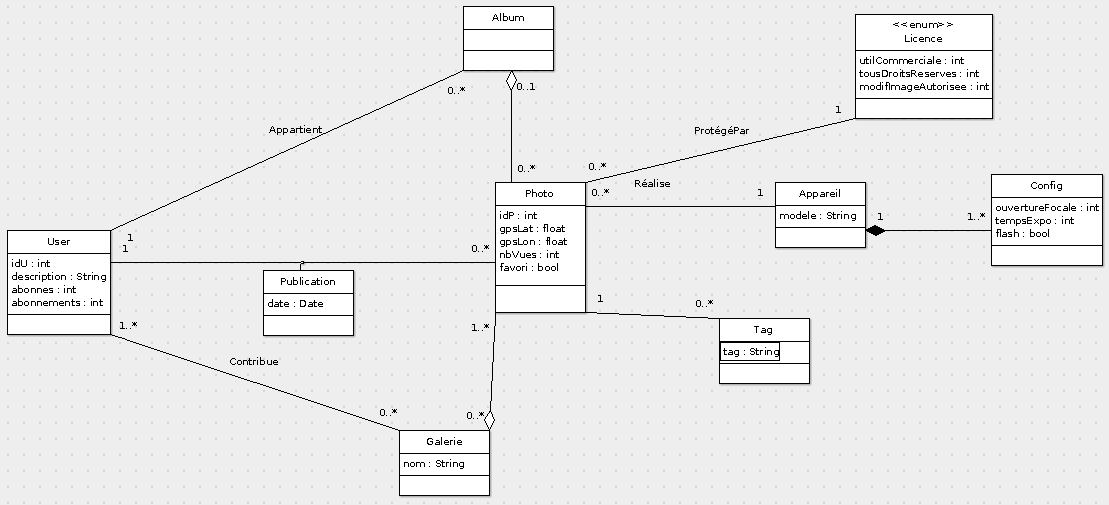
\includegraphics[scale=0.5]{umlTP1.png}
  \end{center}

\subsection{QUESTION 4 :}
  \subsubsection{}

  \begin{DDbox}{\linewidth}

  Photo(\underline{idP: int}, date: Date, gpsLat: float, gpsLon: float, nbVues: int, \textit{idUser: int, idAlbum: int,
  \begin{flushright} idLicence: int, idAppareil: int)\end{flushright}}

  Tag(\underline{idTag: int}, tag: String, \textit{idPhoto: int})\\

  Galerie(\underline{idG: int}, nom: String)\\

  photo\_galerie(\underline{\textit{idPhoto: int, idGalerie: int}})\\

  User(\underline{idU: int}, description: String, preferee : bool, abonnes: int, abonnements:int)\\

  user\_galerie(\underline{\textit{idUser: int, idGalerie: int}})\\

  Appareil(\underline{idAppareil: int}, modeleAppareil: String)\\

  Config(\underline{idConfig: int}, ouvertureFocale: int, tempsExpo: int, flash: bool, \textit{idAppareil: int})\\

  Licence(\underline{idLicence: int}, licence: enum)\\


  \end{DDbox}

  \subsubsection{} Notre modèle ne paraît violer ni la 2NF ni la 3NF.

  \subsubsection{}
    a- violation 2NF: déplacer gpsLat de Photo en attribut de Photo\_galerie: gpsLat ne dépendra que d'une partie de la clef primaire  (ipPhoto).\\
    b- violation 3NF : deplacer l'attribut abonnés de User dans Photo: Abonnes dependra donc de la clef etrangere idUser, qui ne fait pas partie de la clef primaire.

\subsection{QUESTION 5 :}
  \subsubsection{a)}
  \begin{DDbox}{0.4}
   \begin{lstlisting}
SELECT * FROM Photo WHERE gpsLat = 43.62505 AND gpsLon = 3.862038;
SELECT * FROM User, Appareil WHERE User.idAppareil = Appareil.idAppareil AND description = "fan de pingouins" AND modeleAppareil = "KODAC Pingouin"; // Tous les Utilisateurs fan de pingouins possédant un Appareil "KODAC Pingouin"
SELECT COUNT(*) FROM User, Galerie, user_galerie WHERE User.idU = user_galerie.idUser AND user_galerie.idGalerie = Galerie.idGalerie AND Galerie.nom = "Montpellier" GROUP BY idU; // Compte le nombre d'utilisateurs ayant une galerie nommée "Montpellier"
\end{lstlisting}
  \end{DDbox}

  \subsubsection{ b)}
    \begin{DDbox}{0.4}
      \begin{lstlisting}
          SELECT idP FROM Photo, Licence WHERE Licence.idP = Photo.idP AND Licence.licence = "Tous droits réservés" AND nbV > (SELECT AVG(nbVues) FROM Photo);
      \end{lstlisting}
    \end{DDbox}

  \subsubsection{ c)}
  \begin{DDbox}{0.4}
    \begin{lstlisting}
      SELECT idUser FROM User, Photo, DUAL WHERE User.idU = Photo.idP AND trunc(sysdate)-to_date(date, 'dd/mm/yyyy') DAYS > 365*5 GROUP BY idUser;
    \end{lstlisting}
  \end{DDbox}
  \subsubsection{ d)}
  \begin{DDbox}{0.4}
    \begin{lstlisting}
      SELECT COUNT(idGalerie) FROM Photo, photo_galerie WHERE Photo.idP = photo_galerie.idPhoto GROUP BY idPhoto ORDER BY COUNT(idGalerie) DESC LIMIT 5;
    \end{lstlisting}
  \end{DDbox}
  \subsubsection{ e)}
  \begin{DDbox}{0.4}
    \begin{lstlisting}
      SELECT idUser FROM User, Galerie, Photo, photo_galerie, Album WHERE
      User.idUser = Photo.idUser AND
      Photo.idP = photo_galerie.idPhoto AND
      photo_galerie.idGalerie = Galerie.idGalerie AND
      Photo.idAlbum = Album.idAlbum AND
      Galerie.nom = Album.nom;
    \end{lstlisting}
  \end{DDbox}
\section{TP2}
  \subsection {Question 1:}
    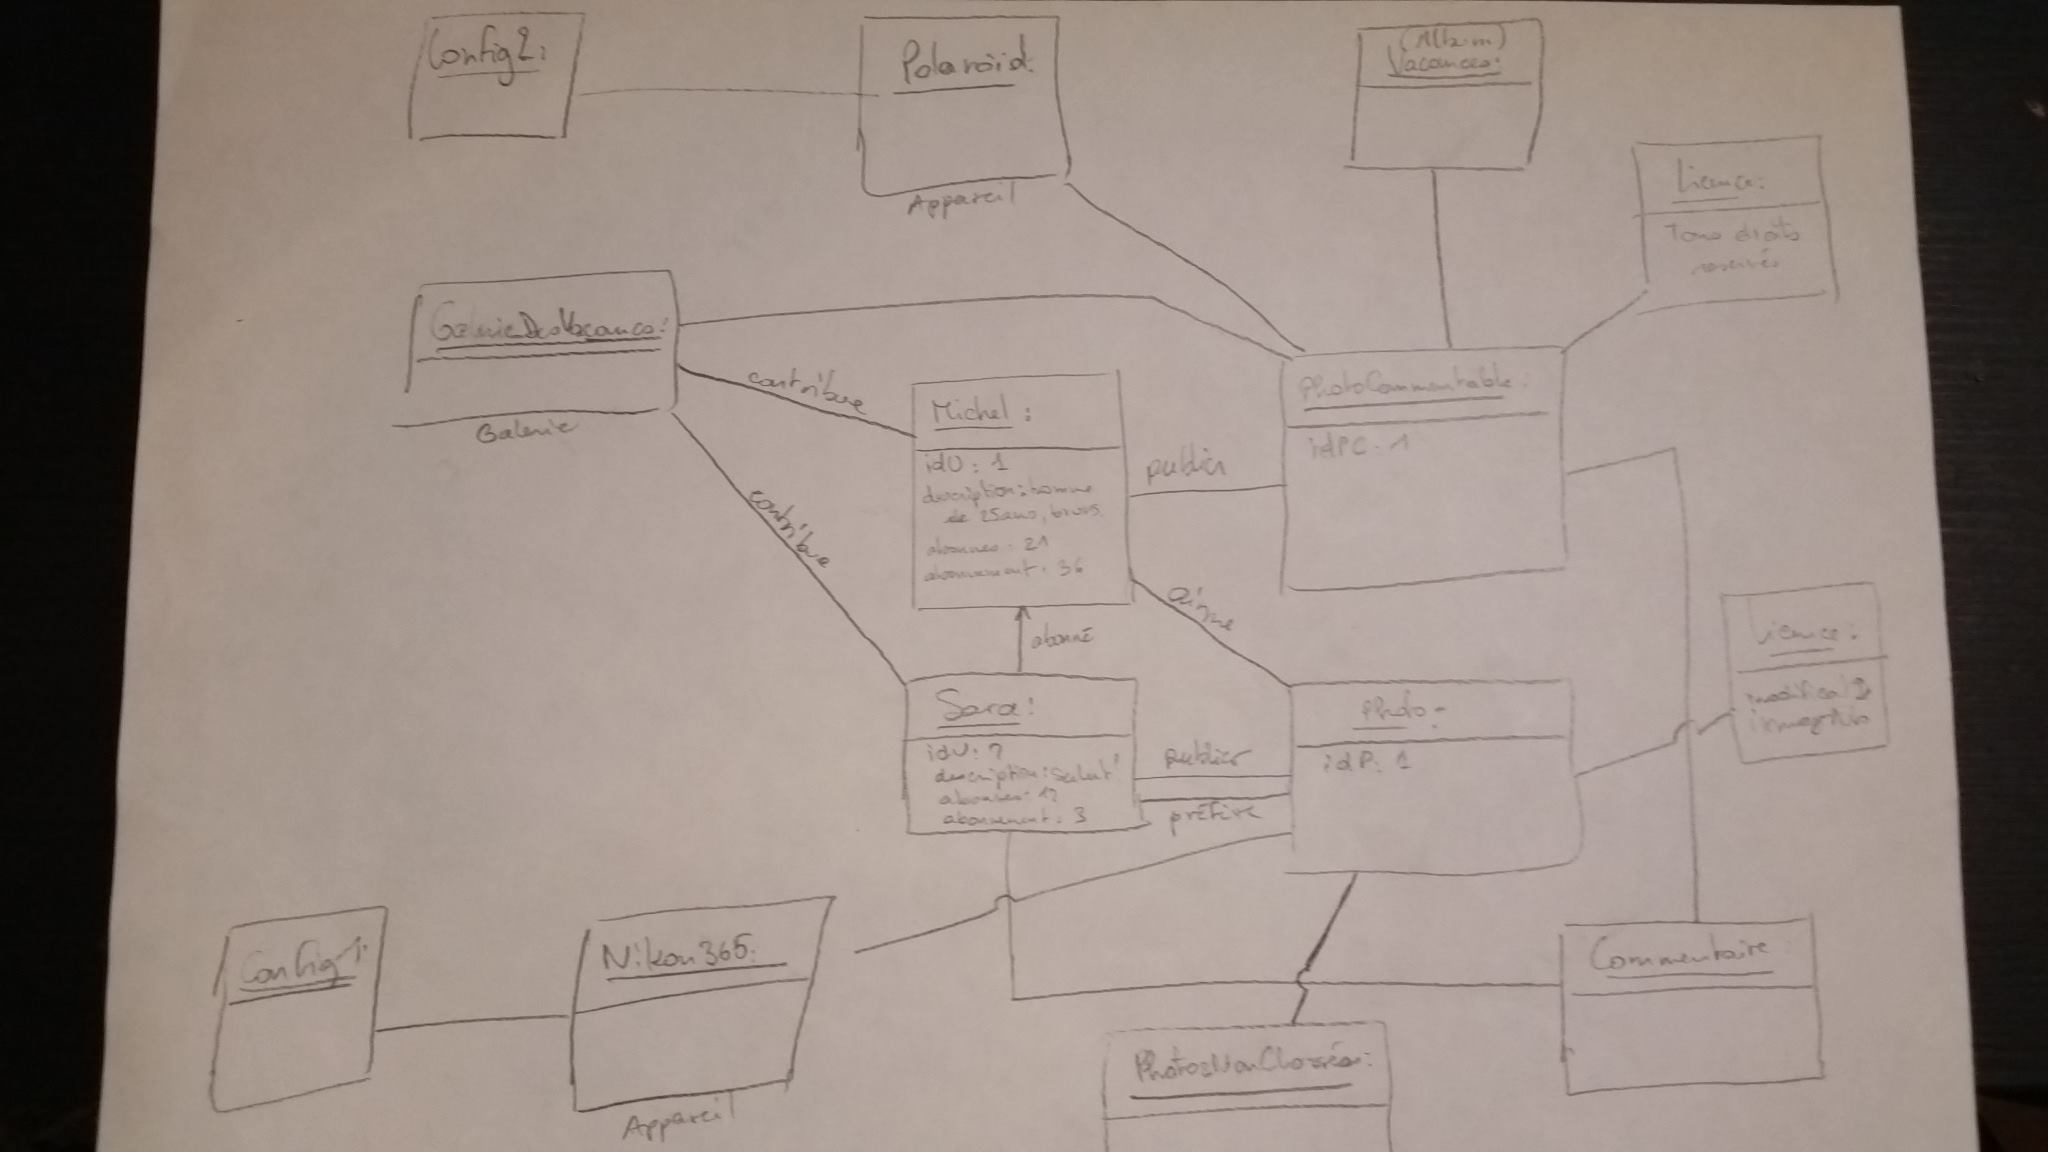
\includegraphics[scale=0.25]{instanciation.jpg}
  \subsection{Question 2:}
    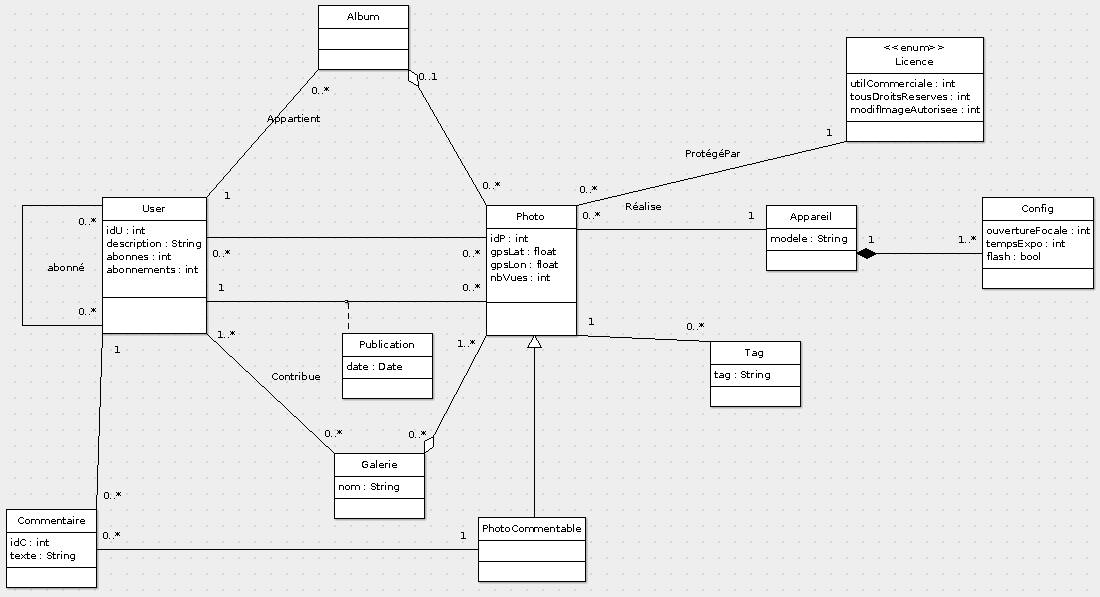
\includegraphics[scale=0.4]{umlTP1-2.png}
    \newpage
    \subsection{Question 4:}
    Le modèle relationnel reprend le même que celui du TP1, avec les ajouts suivants:\\
    \\
      user\_photo\_aime(\underline{\textit{idUser: int, idPhoto: int}})\\
      \\
      abonneA(\underline{\textit{idUser1: int, idUser2: int}})\\
      \\
      commentaire(\underline{idCommentaire: int}, texte: String, date: Date,\textit{ idUser: int})\\
      \\
      PhotoCommentable(\underline{idPC: int}, date:Date, gpsLat: float, gpsLon: float, nbVues: int,\textit{ idUser: int, idAlbum: int, \begin{flushright}idLicence: int, idAppareil: int})\end{flushright}
\end{document}
